\documentclass[11pt]{article}

\usepackage{cite}
\usepackage{comment} %multiline comment
\usepackage{graphicx}
\usepackage{caption}
\usepackage{refstyle}
\usepackage[top=1in, bottom=1in, left=1in, right=1in]{geometry}

\title{Content Based Image Retrieval: Multiple Features Comparative Study }	

\author{
Nora Youssef $^1$,
Alsayed Algergawy  $^2$,
Ibrahim F. Moawad $^1$,
EL-Sayed M. EL-Horbaty $^1$
}

\begin{document}
\maketitle

%\tableofcontents
	
\begin{abstract}
	Multimedia resources are growing rapidly with a huge increase of visual contents. Thus, Searching these images accurately, and efficiently for all types of datasets becomes one of the most challenging tasks. Text-based image retrieval (TBIR) methods involve searching images based on their metadata. Disadvantages of this approach they require huge labor of manual annotation, have been annotated subjectively, limit the search process to metadata, and finally have the synonymy problem. Content-based image retrieval (CBIR) could be a solution for these problems, where it retrieves images based on its visual contents. This paper presents a CBIR system that extends the LIRe open source project in biodiversity domain. The proposed system has four main contributions. Firstly, it generalizes LIRe’s crawler to work on ImageNet synsets. Secondly, to speed LIRe’s crawler parallel approach has been included. Thirdly, extends the LIRe’s analyzer part by implementing new image feature extractors. Finally, it enhances retrieval accuracy by combining multiple features. The proposed system has been evaluated on the ImageNet subset and the experimental results show that the crawling process has been increased by 2.9 times and the retrieval accuracy has been enhanced using the combined features.
\end{abstract}


\footnotetext[1] {Faculty of Computer and Information Sciences, Ain Shams University, Egypt, \{nora.youssef, ibrahim.moawad, s.horbaty \}@cis.asu.edu.eg}

\footnotetext[2]{Friedrich-Schiller University of Jena, Germany,  alsayed.algergawy@uni-jena.de}

\section{Introduction}	

Different forms of multimedia resources (i.e. text, images, audio, and videos) are rapidly growing with a huge development of visual contents and technologies, e.g. data visualized in smart phones, 2D/3D applications, web content, telecommunication, etc. The new century has witnessed an evolution in the amount, availability, complexity, variety and importance of images in all domains. Thus, images play an essential role in a wide range of applications and fields such as education, medical care and social media. However, visual media require a considerable amount of processing and storage, which requires a highly efficient method to index, store, analyze, and retrieve visual information from image databases. Moreover, images have a little metadata by which they can be indexed and searched conveniently.  Consequently, searching images rapidly, accurately, and efficiently for all types of image datasets becomes one of the most challenging tasks \cite{alzu2015semantic}.

The traditional image retrieval techniques are text based image retrieval (TBIR). So that, users can retrieve images based on keywords or textual descriptions which are annotated by human. TBIR systems have main drawbacks (1) huge human labor for the manual annotation, as when a giant data stores are taken into consideration. (2) The subjectivity of the annotation which affects the retrieval accuracy badly, i.e. captions or any other metadata are entered manually. (3) The search is limited to the image text metadata which could produces false negative i.e. if an image misses a part of the metadata or false positive results i.e. f an image contains a wrong metadata, both cases may probably happen by mistake. In addition, a word could have different meanings like “Jaguar” it may be an animal or a car, which would defiantly affect the search results \cite{alzu2015semantic, won2002efficient, jalab2011image, srinivas2015content}.

The term content-based image retrieval (CBIR) appears to have been first used in the literature by Kato [1992] to describe his experiments in the automatic retrieval of images from a database by color and shape. \cite{jalab2011image} CBIR has been introduced as a solution for the TBIR limitations, it is considered as, the technique of effective retrieval of images from an oversized data store \cite{alzu2015semantic, won2002efficient, jalab2011image, srinivas2015content}. The typical CBIR system performs two major tasks. The first one is feature extraction, where a set of features is extracted to describe the content of each image in the database. The second task is the similarity measurement between the query image and each image in the database, using the feature extraction. The feature extraction values for a given image are stored in a descriptor that can be used for retrieving similar images. Image descriptors are descriptions of the visual features of the contents in images that produce such descriptions. They describe elementary characteristics, such as color, texture, shape and spatial location \cite{jalab2011image}. There are various examples of CBIR systems: LIRe \cite{lux2011content}, VisualSeek \cite{smith1997visualseek} and SIMPLicity \cite{wang2001simplicity}.

The proposed is a CBIR for biodiversity domain. It has two main objectives, in other words, two main modifications of LIRe system. On one hand, crawler modification: firstly by replacing the flickr dataset by a dataset that suits the biodiversity domain. Secondly, the dataset is fed into the system via a user input. Finally, increase the crawler speed. The second main objective is to enhance the retrieval quality by building the image descriptor by a mixture of different image features. The rest of the paper is organized as: Section 2, related work. Section 3, introduces the LIRe system in details. Section 4, proposes the methodology and how the LIRe system has been customized. Section 5, the discussion and the experimental results. In addition the system evaluation. Finally section 6, concludes the paper.

\begin{figure}[h]
\centering
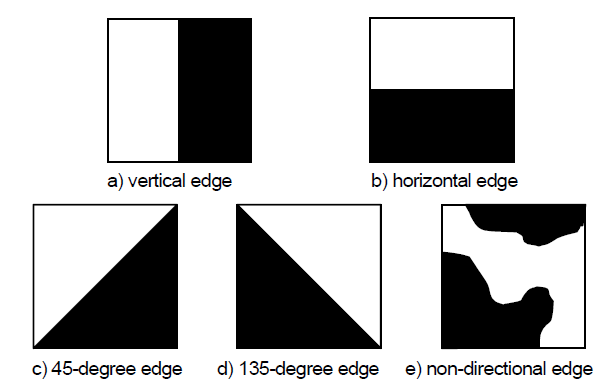
\includegraphics[width=0.3\textwidth]{edgesTypes}
\caption{Five edges types}.
\label{fig:edgesTypes}
\end{figure}

\section{Image Descriptors}

Visual image descriptors or image low level features are descriptions of the visual contents in an image or video. They are algorithms or applications that produce such descriptions. They describe elementary characteristics such as the shape, the color, the texture, edge or spatial location \cite{goshtasby2012image}. Thus, feature extraction and representation is a an important step for multimedia processing \cite{Tian2013ARO}. Histogram is the most commonly used structure to represent any global feature composition of an image. It is invariant to image translation and rotation, it is also considered a very useful for indexing and retrieving images \cite{Dr2010EfficientUO, park2000efficient, balasubramani2009efficient}. In this paper we will focus on edge, color and fuzzy color texture histogram and the combination among them.

\begin{figure}[h]
\centering
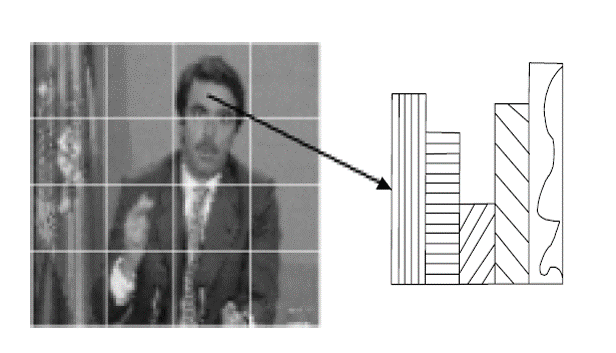
\includegraphics[width=0.4\textwidth]{edgesInImageSubBlock}
\caption{Five edges types}.
\label{fig:edgesInImageSubBlock}
\end{figure}

\subsection{Edge Histogram Descriptor (EHD)}
Edge in image is an important low-level feature. It can describe both shape and texture features, which are essential elements for content-based image analysis \cite{won2004feature, balasubramani2009efficient}. The Edge Histogram Descriptor (EHD) describes five edge types in the image,namely horizontal,vertical,two diagonal and non-directional edge types as shown in figure \ref{fig:edgesTypes}. Population for these five types of edges in a local image region of a sub-image is represented by a histogram with five bins. Specifically, the image space is divided into 16 (4×4) non-overlapping sub-images and for each sub-image a histogram with five edge bins is generated as in figure \ref{fig:edgesInImageSubBlock}, yielding a combined edge histogram with 80 (16×5) bins for the entire image. The histogram with 80 bins is the standardized edge descriptor for MPEG-7, figure visualizes the EHD \ref{fig:EDH} \cite{won2002efficient, won2004feature, lisin2005combining, park2000efficient}.


\begin{figure}[h]
\centering
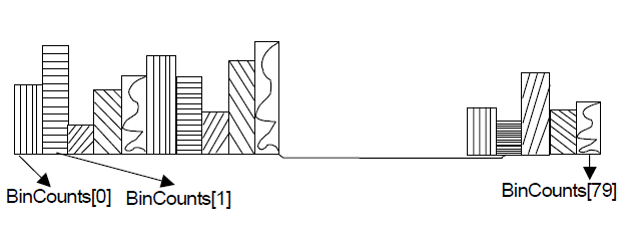
\includegraphics[width=0.4\textwidth]{EDH}
\caption{Edge Descriptor Histogram }.
\label{fig:EDH}
\end{figure}

However, using the local histogram bins only may not be sufficient to represent global features of the edge distribution. Thus, to improve the retrieval performance, we need global edge distribution as well. On one hand, the global edge histogram is a 5 bin histogram and it can be calculated by the summation of the same type of edge in the corresponding bins in local edge histogram as shown in figure \ref{fig:globalEDH} \cite{won2002efficient, won2004feature, lisin2005combining, park2000efficient}.

\begin{figure}[th]
\centering
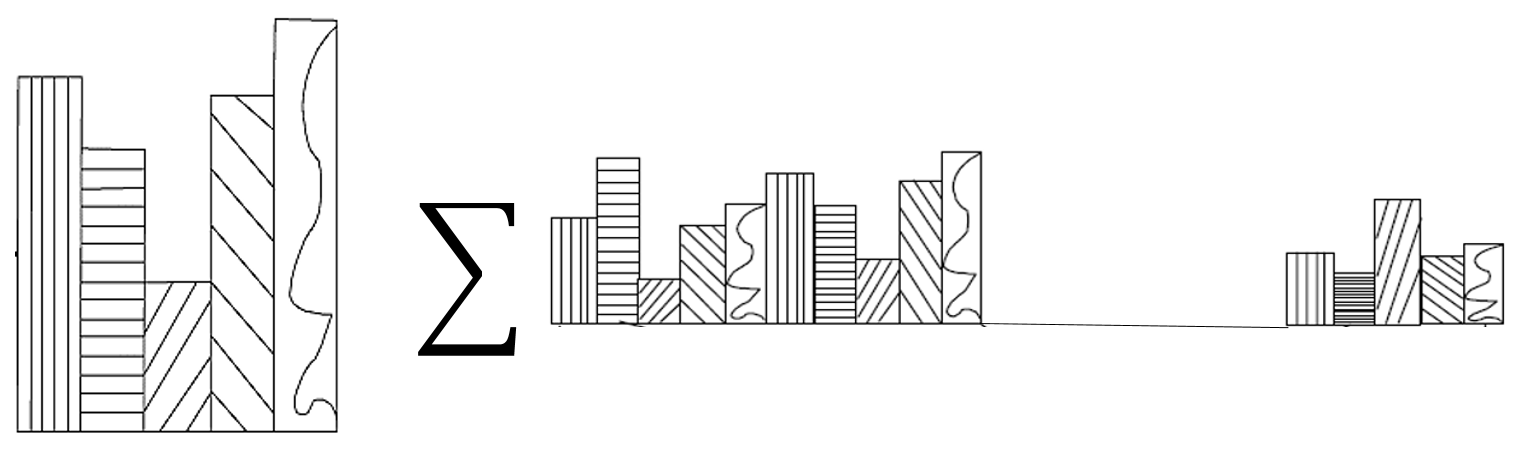
\includegraphics[width=0.4\textwidth]{globalEDH}
\caption{Global Edge Descriptor Histogram}.
\label{fig:globalEDH}
\end{figure}

On the other hand, the semi-global histogram could be generated as shown in figure \ref{fig:semiGlobalEDH} and it will yield 65 bin histogram. By using the combination of the three types edge, we would have a 150 (80 + 5 + 65) bin edge histogram. Finally the distance between 2 combined edge histograms would be given by equation \ref{eq:combinedEdgeHistogramDistance}.

\begin{equation}\label{eq:combinedEdgeHistogramDistance}
  D(A,B) = \sum_{k = 0}^{79}{| Local_{A[i]} - Local_{B[i]}|} + 5 \sum_{k = 0}^{4}{| Global_{A[i]} - Global_{B[i]}|} + \sum_{k = 0}^{64}{| Semi\_Global_{A[i]} - Semi\_Global_{B[i]}|}
\end{equation}


\begin{figure}[h]
\centering
\includegraphics[width=0.4\textwidth]{semiGlobalEDH}
\caption{Semi-Global Edge Descriptor Histogram}.
\label{fig:semiGlobalEDH}
\end{figure}


\subsection{Color Layout Descriptor (CLD)}

Color is one of the most important features of images. Color features are defined subject to a particular color space or model. A number of color spaces have been used in literature, such as RGB and HSV \cite{goshtasby2012image}. For instance, the CLD is used in representation of the spatial distribution of colors in images. It is a compact descriptor that consists of representative colors and it is encoded using a non-overlay 8 x 8 sliding window over an color image followed by performing a Discrete Cosine Transform (DCT)\cite{tsai2016design, balasubramani2009efficient}. Figure \ref{colorLayoutExample} visualizes an example for color layout.


\begin{figure}[h]
\centering
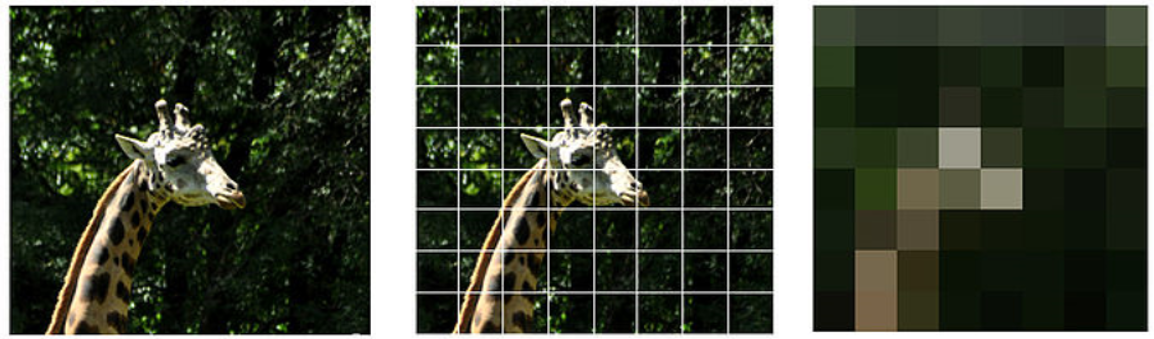
\includegraphics[width=0.4\textwidth]{colorLayoutExample}
\caption{Visualization for color layout descriptor}.
\label{fig:colorLayoutExample}
\end{figure}


 Color layout (CLD) could be combined with other features for better retrieval accuracy. It could be combined with Gabor filter in wavelet domain for texture description \cite{jalab2011image}. Another idea proposed by \cite{tsai2016design}, they combined a mixture of three color features at the same time for image retrieval, these features are dominant color (DCD), SCD that is like the traditional color histogram but in HSV color space and CLD. One more idea by \cite {balasubramani2009efficient} is to merge the CLD with EHD. In this paper, CLD have integrated with the combined edge histogram (Local + Global + Semi-Globa) for image retrieval and the similarity is calculated as in equation \ref{colorLayoutCombinedEdgeSim}

 \begin{equation}\label{eq:colorLayoutCombinedEdgeSim}
  D(A,B) = \sum_{k = 0}^{79}{| Local_{A[i]} - Local_{B[i]}|} + 5 \sum_{k = 0}^{4}{| Global_{A[i]} - Global_{B[i]}|} + \sum_{k = 0}^{64}{| Semi\_Global_{A[i]} - Semi\_Global_{B[i]}|} +
  \sum_{k = 0}^{63}{| YCoeff_{A[i]} - YCoeff_{B[i]}|} + \sum_{k = 0}^{63}{| CbCoeff_{A[i]} - CbCoeff1_{B[i]}|} + \sum_{k = 0}^{63}{| YCoeff_{A[i]} - YCoeff_{B[i]}|} + \sum_{k = 0}^{63}{| CrCoeff_{A[i]} - CrCoeff1_{B[i]}|}
\end{equation}

Such that $Local_{A,B}$, $Global_{A,B}$ and $Semi\_Global_{A, B}$ are for combined edge histogram. On the other hand, the $YCoeff_{A,B}$, $CbCoeff_{A,B}$ and $CrCoeff_{A,B}$ are for the CLD.

\subsection{Fuzzy Color Texture Histogram (FCTH)}

\section{Experimental Evaluation}

\begin{figure}[h]
\centering
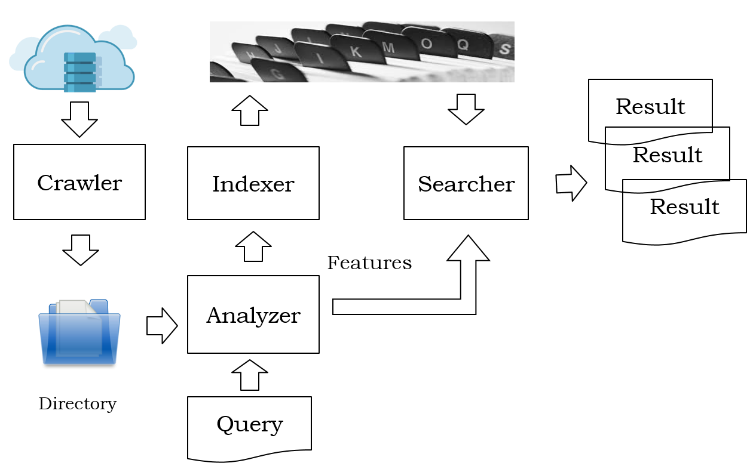
\includegraphics[width=0.5\textwidth]{lireBlockDiagram}
\caption{LIRe Block Diagram}.
\label{fig:lireBlockDiagram}
\end{figure}

\subsection{LIRE System}

LIRE (Lucene Image Retrieval) is an open source library for content based image retrieval, which means you can search for images that look similar. Besides providing multiple common and state of the art retrieval mechanisms LIRE allows for easy use on multiple platforms \cite{lux2011content}. LIRe with its default architecture does not suit the biodiversity domain very well. This is due to the very general data-set which is just a collection of random images from the filckr data-set and the downloaded images don't relate to the biodiversity field. In addition we found the crawler is slow to some extent and this would be an issue at the biodiversity field, because we are usually dealing with huge data-sets. The analyzer extracts only one image feature at a time and the searcher measure the distance between the query image and the data-set against only one feature value, but as shown at \cite{ping2013review, won2002efficient, park2000efficient, won2004feature} we may mix multiple features at a time for better image description. Thus, we can enhance the retrieval accuracy.

The main components of the LIRe system is given by \figref{lireBlockDiagram} which represents its block diagram. These components are: crawler, indexer, analyzer and searcher. Such that, the crawler craps a random number of images from the flickr dataset and save these downloaded images into a local directory/folder. The analyzer component extracts the images features using the state-of-the-art methods as mentioned above. The third component is the indexer component which takes the extracted image features and build a Lucene based index. The last component searcher or matcher takes the query image and calculate the distance or the similarity between the input and the images that are stored in the index, it then displays the most relevant images.

\subsection{Evaluation Criteria}

Precision and recall, F measure and mean average precision $mAP$ are the basic measures that are used in evaluating search strategies. Assumes that there are two sets as in figure \ref{fig:measurements}. The one on the right gives the set of items retrieved and the set on the left gives the set of relevant items for a query in the database. This gives the next three notations.
\begin{itemize}
\item{A: Relevant items that were retrieved. }
\item{B: Relevant items that not retrieved. }
\item{C: Irrelevant items that were retrieved. }
\end{itemize}

\begin{figure}[h]
\centering
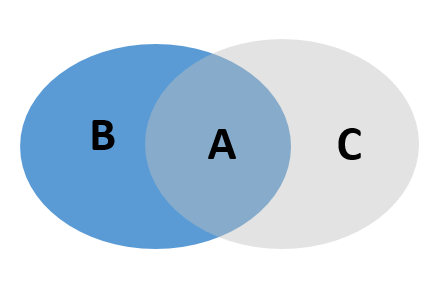
\includegraphics[width=0.3\textwidth]{measurements}
\caption{Precision and recall measurements illustration.}
\label{fig:measurements}
\end{figure}

Precision: Equation \ref{eq:Pr} gives the ratio of the number of relevant
records retrieved to the total number of irrelevant and
relevant records retrieved. It is usually expressed as a
percentage.

	\begin{equation}\label{eq:Pr}	
	  Pr = \frac{A}{A + C}
	\end{equation}
	
Recall: Equation \ref{eq:R} gives the ratio of the number of relevant items
retrieved to the total number of relevant items in the
database. It is usually expressed as a percentage.

	\begin{equation}\label{eq:R}
	  R = \frac{A}{A + B}	
	\end{equation}
	
F allows to trade off precision against recall.	 In this paper the balanced F with $\alpha = 0.5$ has been used.
	\begin{equation} \label{eq:F}
	F = \frac{1}{\alpha \frac{1}{Pr} + (1 - \alpha)\frac{1}{R}}
	\end{equation}


Moreover, the mean average precision $mAP$ is given by equation \ref{eq:mAP} shows the average of precision value of all tested queries.
	\begin{equation} \label{eq:mAP}
	   mAP = \frac{\sum{Pr}}{\#queries}
	\end{equation}

\begin{figure}[h]
\centering
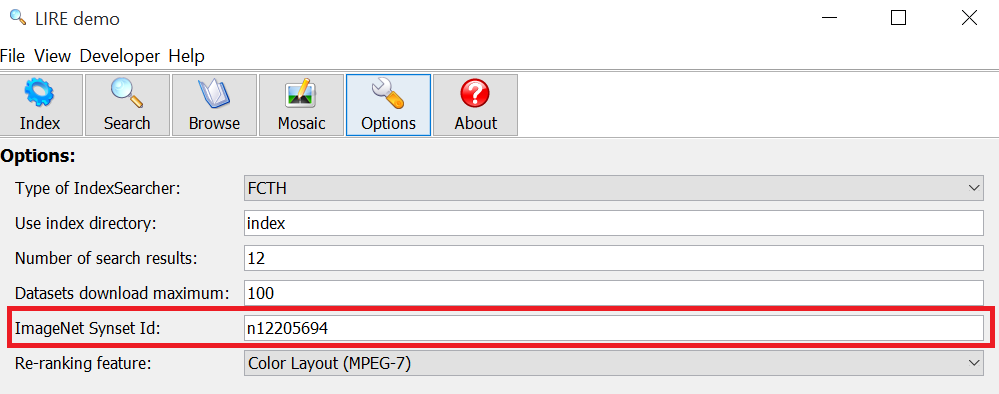
\includegraphics[width=0.6\textwidth]{lireSettingPage}
\caption{LIRe settings page.}
\label{fig:lireSettingsPage}
\end{figure}

\subsection{Dataset and Queries}

ImageNet is an image database organized according to the WordNet hierarchy (currently only the nouns), in which each node of the hierarchy is depicted by hundreds and thousands of images \cite{deng2009imagenet}. In this paper, experiments were done on four different synsets of ImageNet, these synsets are given by table \ref{tbl:synsets}, that it gives an overview about the synsets used in terms of name, synset Id, number or downloaded images and a sample for each of them. The public API for downloading these synsets is given by \texttt{http://www.image-net.org/api/text/imagenet.synset.geturls?wnid=}. while the synset id or wnid is a user input as in figure \ref{fig:lireSettingsPage}.



\begin{table}
\caption{Selected synsets details}
\begin{tabular}{cccc}

		\hline
		Synset & Id & \#Images & Sample \\ \hline
		\\
		Animal & n00015388 & 400 &
		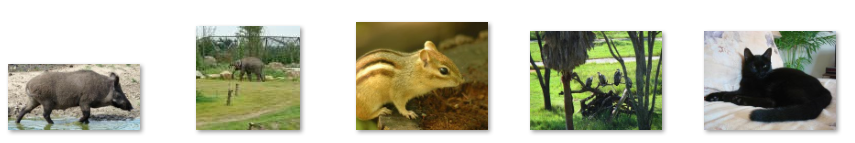
\includegraphics[width=0.5\textwidth]{AnimalSynset}	
		\\
		Planet flora,
		\\ planet life  & n00017222 & 400 &
		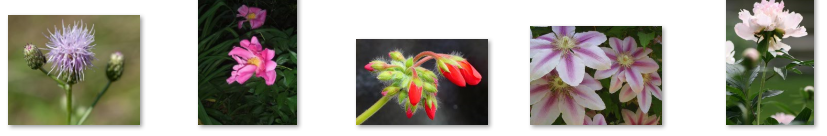
\includegraphics[width=0.5\textwidth]{HerbsSynset}	
		\\
		 Owl  & n01621127 & 100 &
		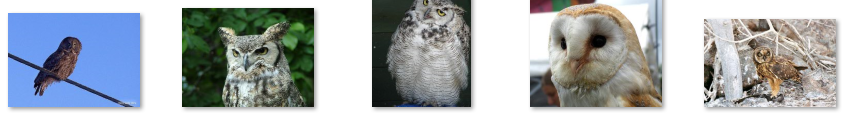
\includegraphics[width=0.5\textwidth]{OwlSynset}	
		\\
			Elephant  & n02503517 & 100 &
		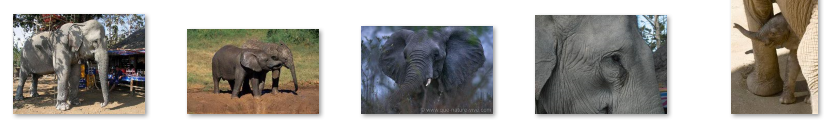
\includegraphics[width=0.5\textwidth]{ElephantSynset}	
		\\ \hline
\end{tabular}

\label{tbl:synsets}
\end{table}

Queries for the experiments are randomly selected that covers all the fours synsets figure \ref{fig:queries} shows a sample for the selected queries.

\begin{figure}[h]
\centering
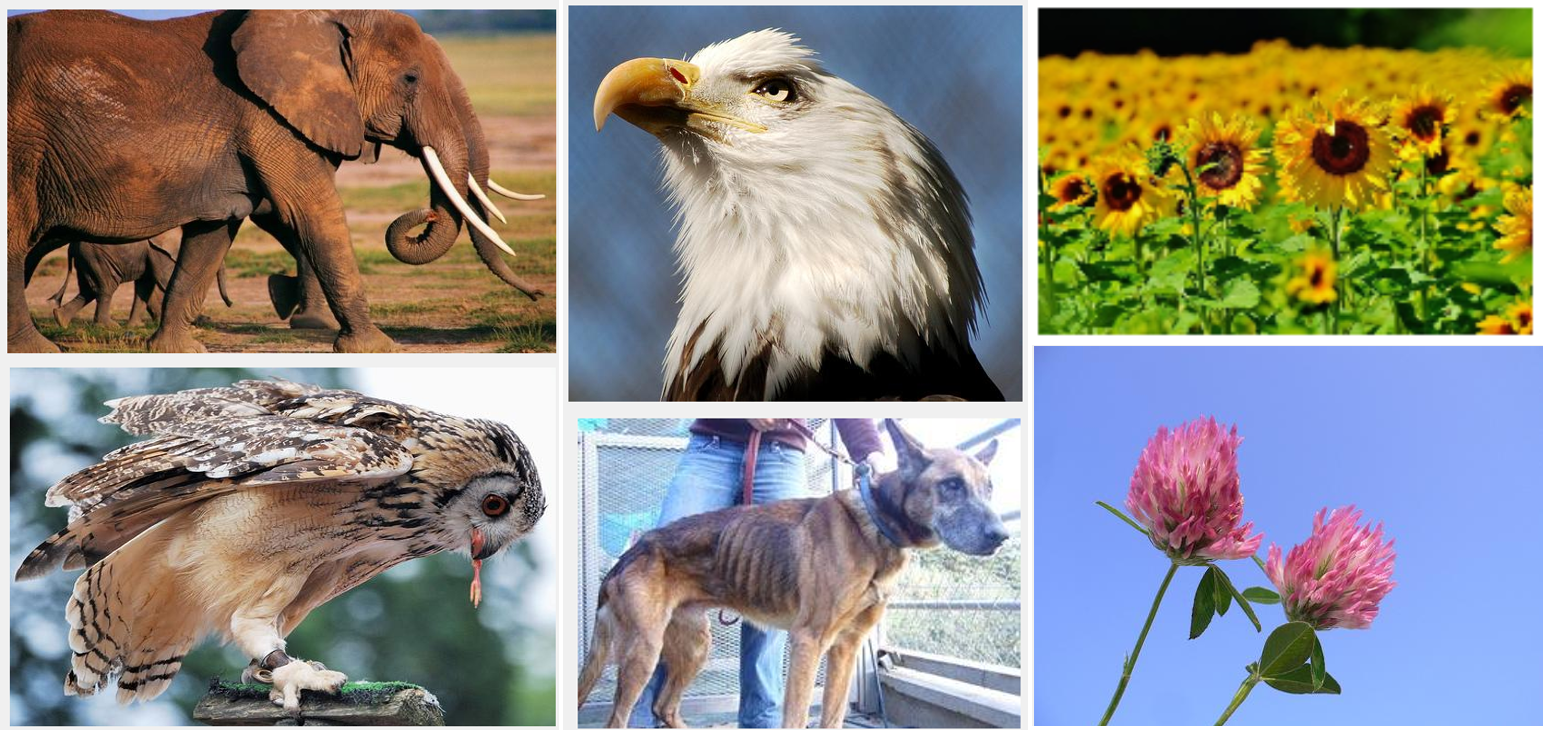
\includegraphics[width=0.5\textwidth]{queries}
\caption{A sample of the selected queries.}
\label{fig:queries}
\end{figure}

\begin{figure}[h]
\centering
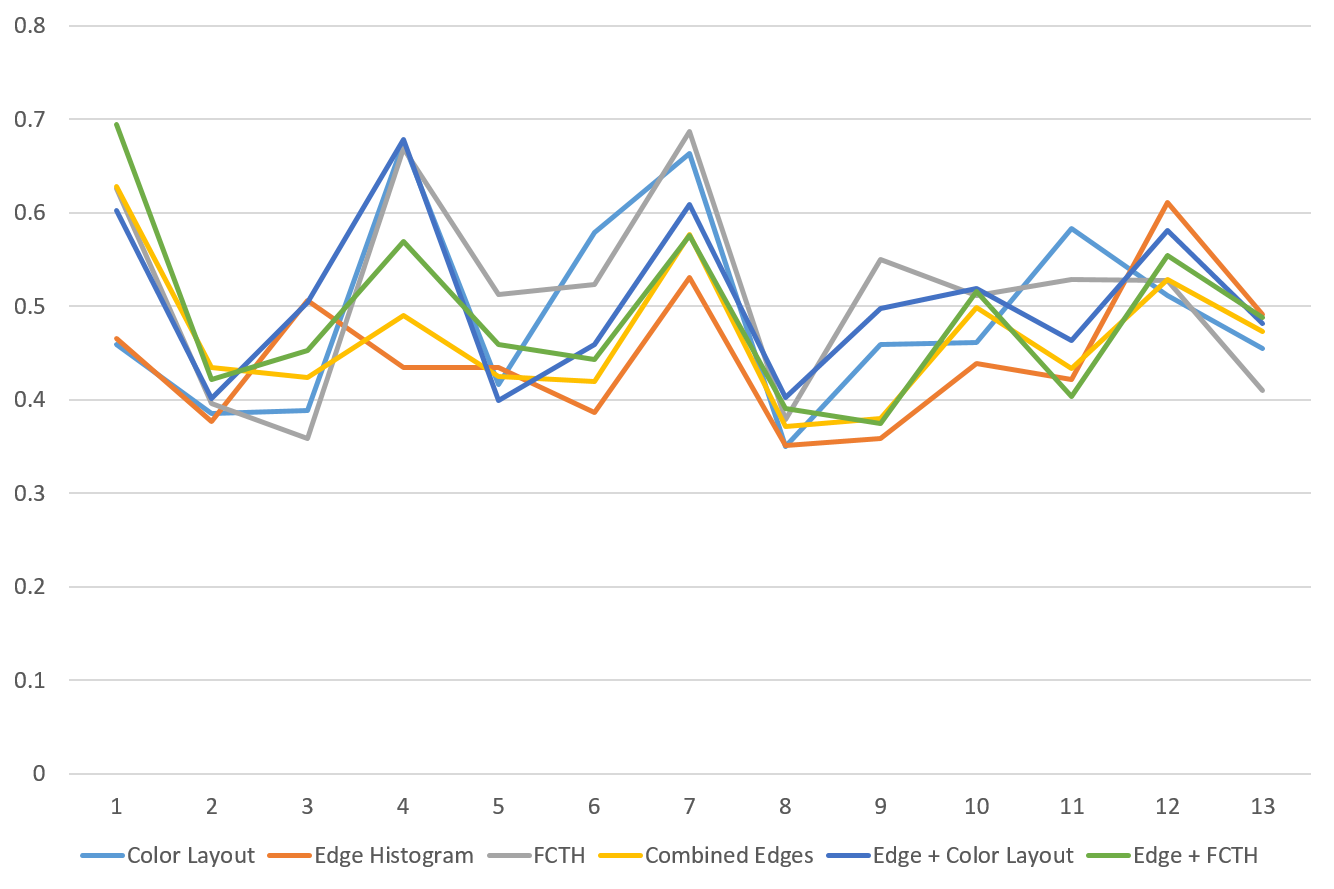
\includegraphics[width=0.9\textwidth]{PrResults}
\caption{ Precision $(pr)$ graph for 6 algorithms and 13 queries.}
\label{fig:PrResults}
\end{figure}

\subsection{Results}

The experiment includes 13 different queries, each of them has been tested against 6 algorithms. On one hand, the state-of-the-art: Color layout, local edge histogram, fuzzy color texture histogram (FCTH). On the other hand: Combined edge histogram, edge histogram and color layout (Edge + Color) and  finally, edge histogram and FCTH (Edge + FCTH).

\begin{figure}[h]
\centering
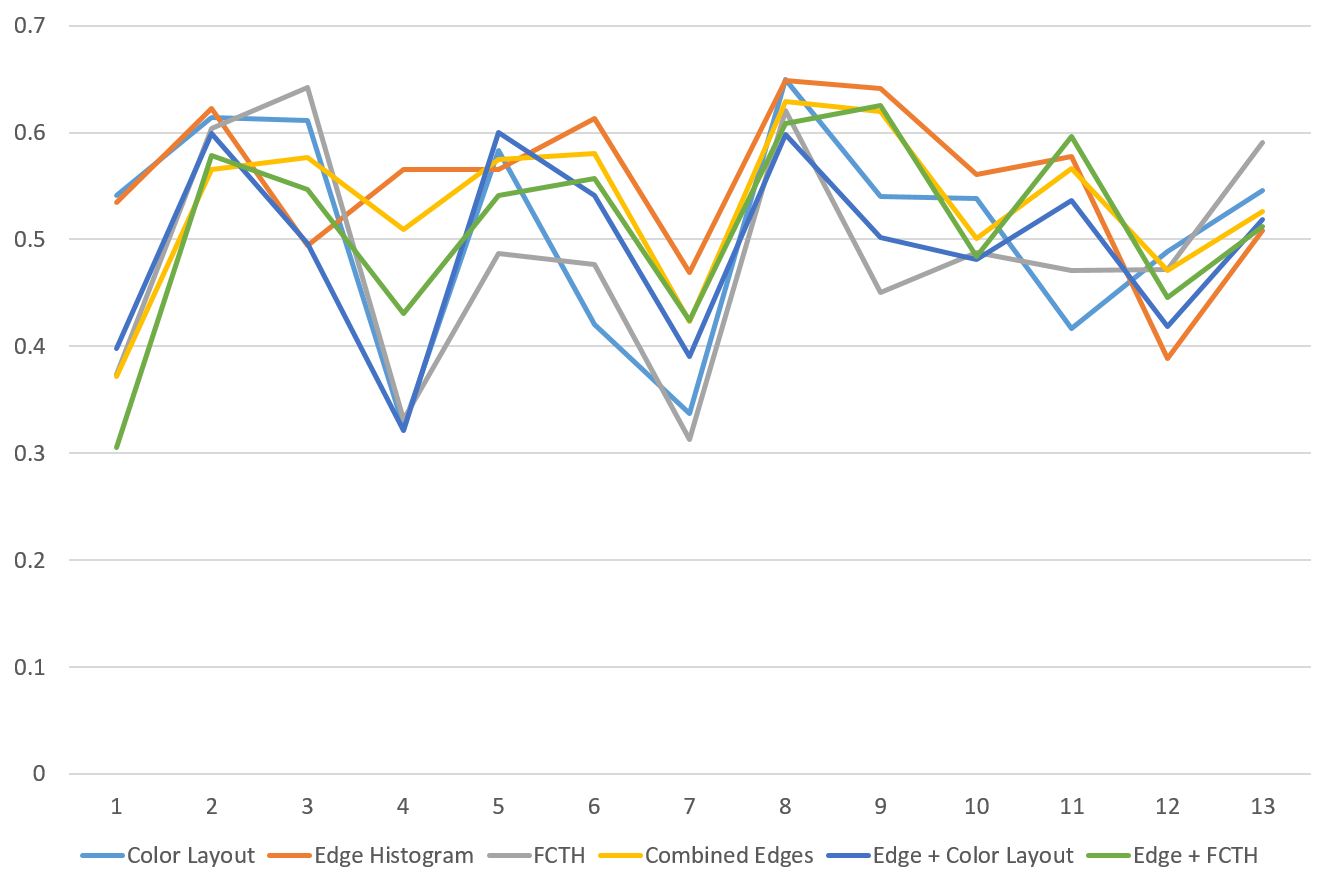
\includegraphics[width=0.9\textwidth]{ResultsRecall}
\caption{ Recall $(R)$ graph for 6 algorithms and 13 queries.}
\label{fig:ResultsRecall}
\end{figure}

Results are shown in terms of precision, recall, F measure graph and mean average precision $mAP$. figure \ref{fig:PrResults} shows the average precision values of 10 users for each one of the 13 queries.

\begin{figure}[h]
\centering
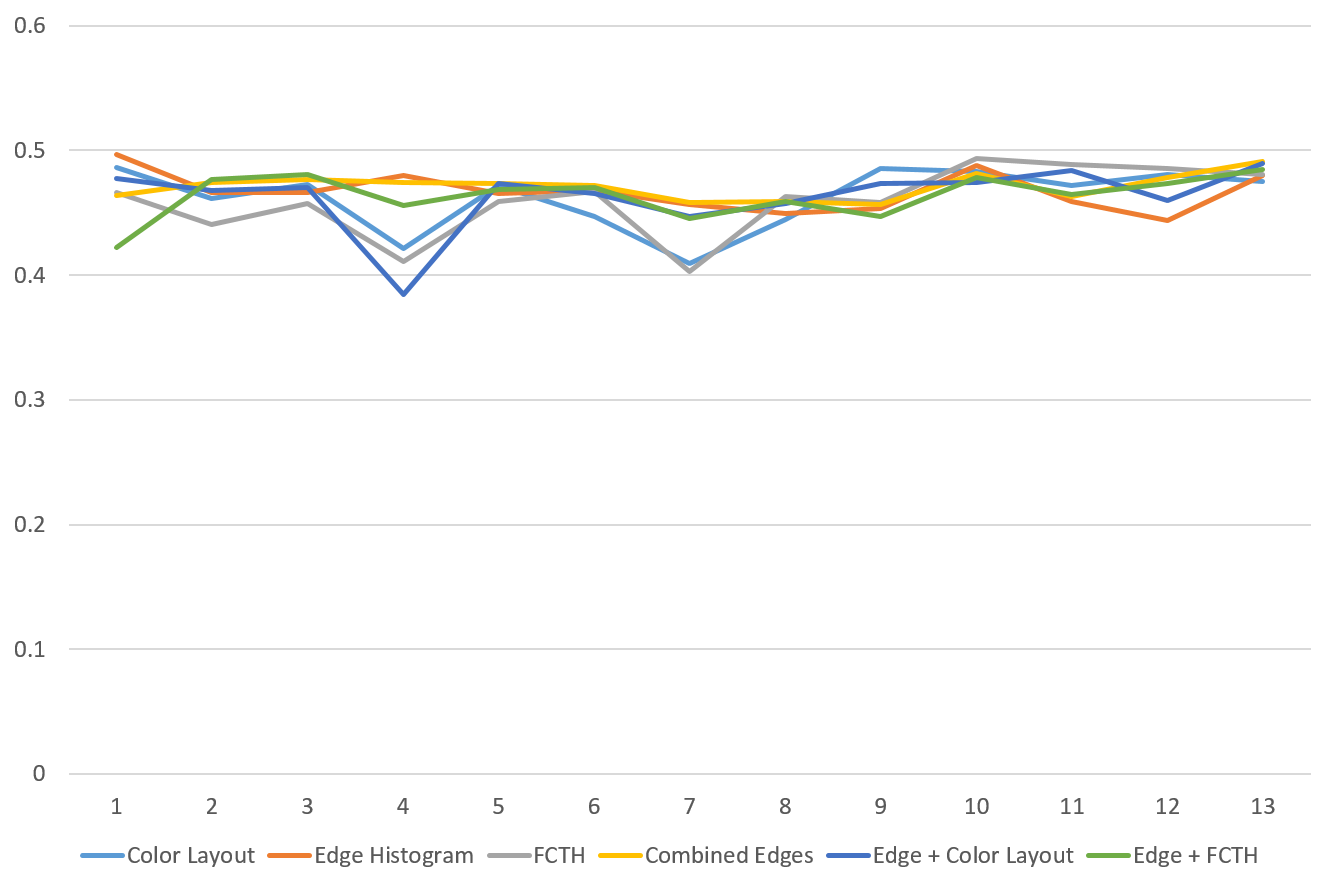
\includegraphics[width=0.9\textwidth]{ResultsF}
\caption{ $F$ Measure.}
\label{fig:ResultsF}
\end{figure}

Query 1, Query 4 and Query 7 belong to “Herbs” and “Elephant Synset”. We have many images that matches the exact color and with duplicates, that’s why the color feature exceeded either in Color or (Edge + Color) combined. FCTH appears as a second rank which color based feature but it takes the texture into consideration as well. In other words, adding something extra feature like edge was not the best option while we have sufficient amount of images that it could be retrieved by single feature. Thus, it actually included some false positives just cause it matches the query's edges.



Query 2 and Query 8 which are 2 queries for a cat and giraffe respectively, as noticed the 6  algorithms gave their minimum $Pr$ values, this is due the lack of images that have either giraffe or a cat there is only 1 and 2 available matches in the downloaded synsets. In other words, this means most of the retrieved results are irrelevant.

\begin{figure}[th]
\centering
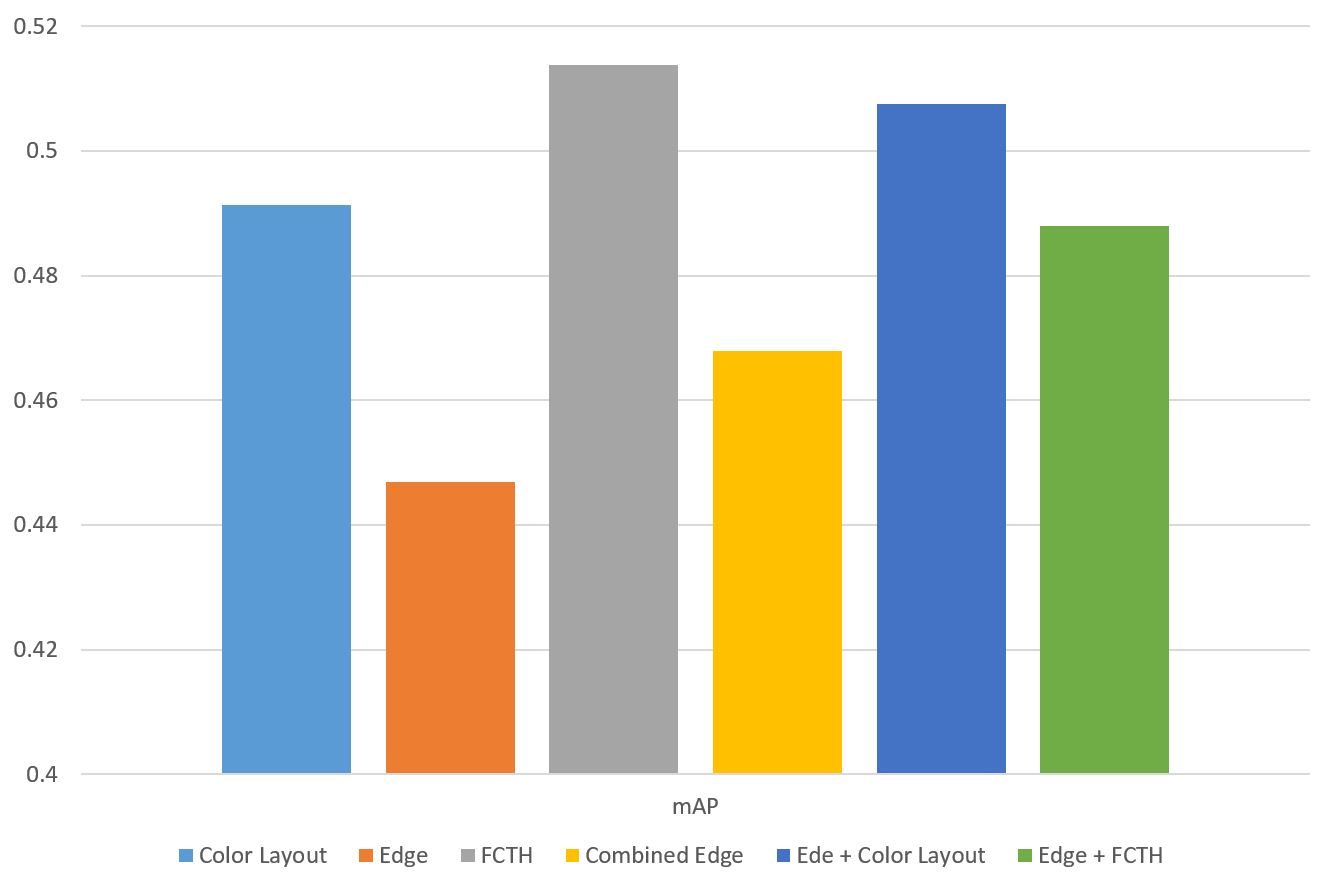
\includegraphics[width=0.9\textwidth]{mAP}
\caption{ $mAP$ chart.}
\label{fig:mAP}
\end{figure}

Figure \ref{fig:ResultsF} shows the average balanced F measure of the 13 queries, such that $\alpha = 0.5$. Moreover, Figure \ref{fig:mAP} shows the $mAP$ for them. It is shown that  using multiple features like combined edges exceeded the local edge histogram and edge + color layout exceeded both of color layout and local edge as  separate features. However, the combination of edge and FCTH exceeded local edge histogram but retreated the FCTH.

\section{Conclusion and Future Work}




\begin{Large}
\textbf{Acknowledgment}
\end{Large}

This work was done at the SWEP course as a part of the BioDialog project which is funded by DAAD at Friedrich Schiller University of Jena. Special thanks Prof.
Birgitta König-Ries for her support.

%References ...
\bibliographystyle{ieeetran}
\bibliography{References/all-references}
\end{document} 